%%%%%%%%%%%%%%%%%%%%%%%%%%%%%%%%%%%%%%%%%%%%%%%%%%%%%%%%%%%%%%%%%%%%%%%%%%%%%%%%
\section{Lecture 6: Paleocene-Eocene Thermal Maximum}

Snowball Earth won't happen again because of vegetation it would be
very hard to get that albedo effect.

The brown section in sediment blocks from Ocean Drilling Program is pure clay,
corresponding to a period without deep marine life.

\textbf{Cenozoic Era} is the last 66 Myr, from the last major extinction to
the present day.

\begin{figure}[H]
    \centering
    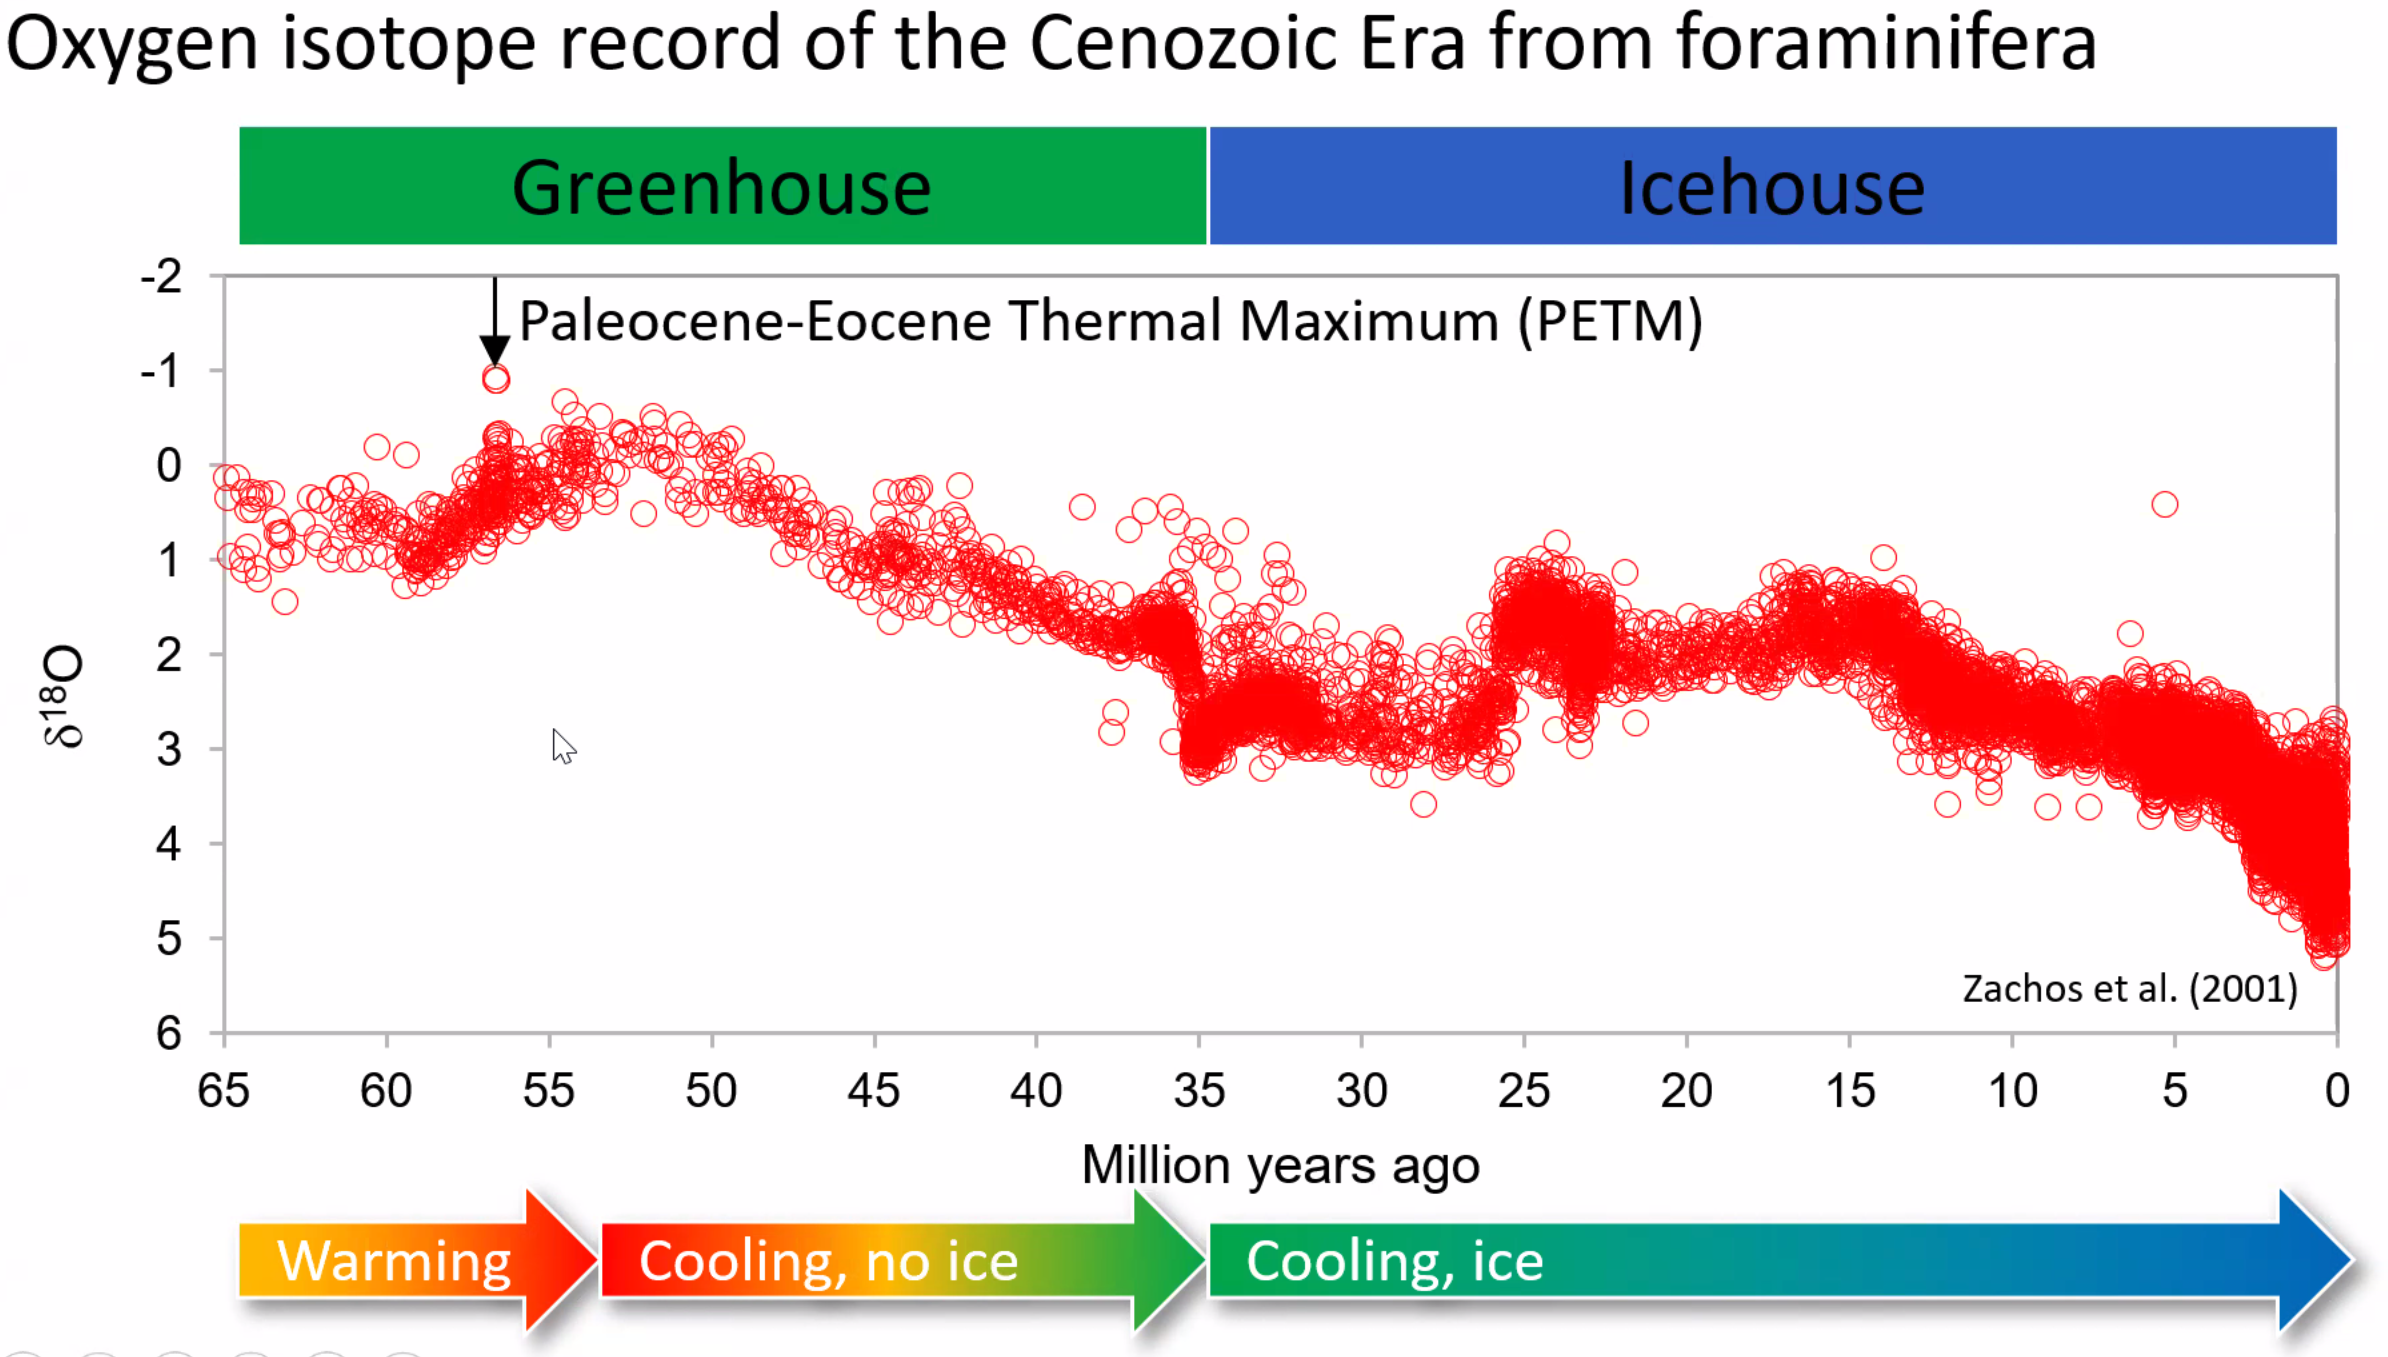
\includegraphics[width=0.95\linewidth]
    {content/img/cenozoic_isotope_record_from_forams.png}
\end{figure}

If we zoom into the above graph, the spike is very sudden, on a scale of 1 Myr.
$\delta^{18}$O changes from 0.5 to -1.

$\Delta T = 4.2[\delta^{18}O_1 - \delta^{18}O_2]$

$\Delta T = 4.2[1.5] = 6.3 \degree$

So what we observe is a temperature change of $+6.3 \degree$. We're currently
experiencing a world $1.5 \degree$ warmer than it should be.

We see the effect of \textbf{extreme warming} in the marine life -- there seems
to be absence of forams sediments in that period of time. The warming is clearly
correlated with a mass extinction.

\subsection{Cerrejon mine, Colombia}

In this coal mine, researchers have found fossils of a snake \textit{titanoboa
cerrejonensis vertebrae}. The snake was \textit{massive}, much bigger than
Boa constrictor (3.4m).

\subsection{Titanoboa cerrejonensis as a paleothermometer}

Modern light green anaconda: 7.3m, living in mean annual temperature of
$27 \degree$C.

Titanaboa was at least 13m, living in $32-33 \degree$C.

(both measured at $5.5\degree$N).

Mean annual temperature at PETM was $39-40 \degree$C.

\subsection{Mean annual temperature and latitude}

In a warmer climate, temperature flattens out. We see it today, we call it
Arctic amplification. In the Arctic regions, warming is happening much faster
then elsewhere. In Svalbard, there's up to 10 degrees of warming.

\begin{figure}[H]
    \centering
    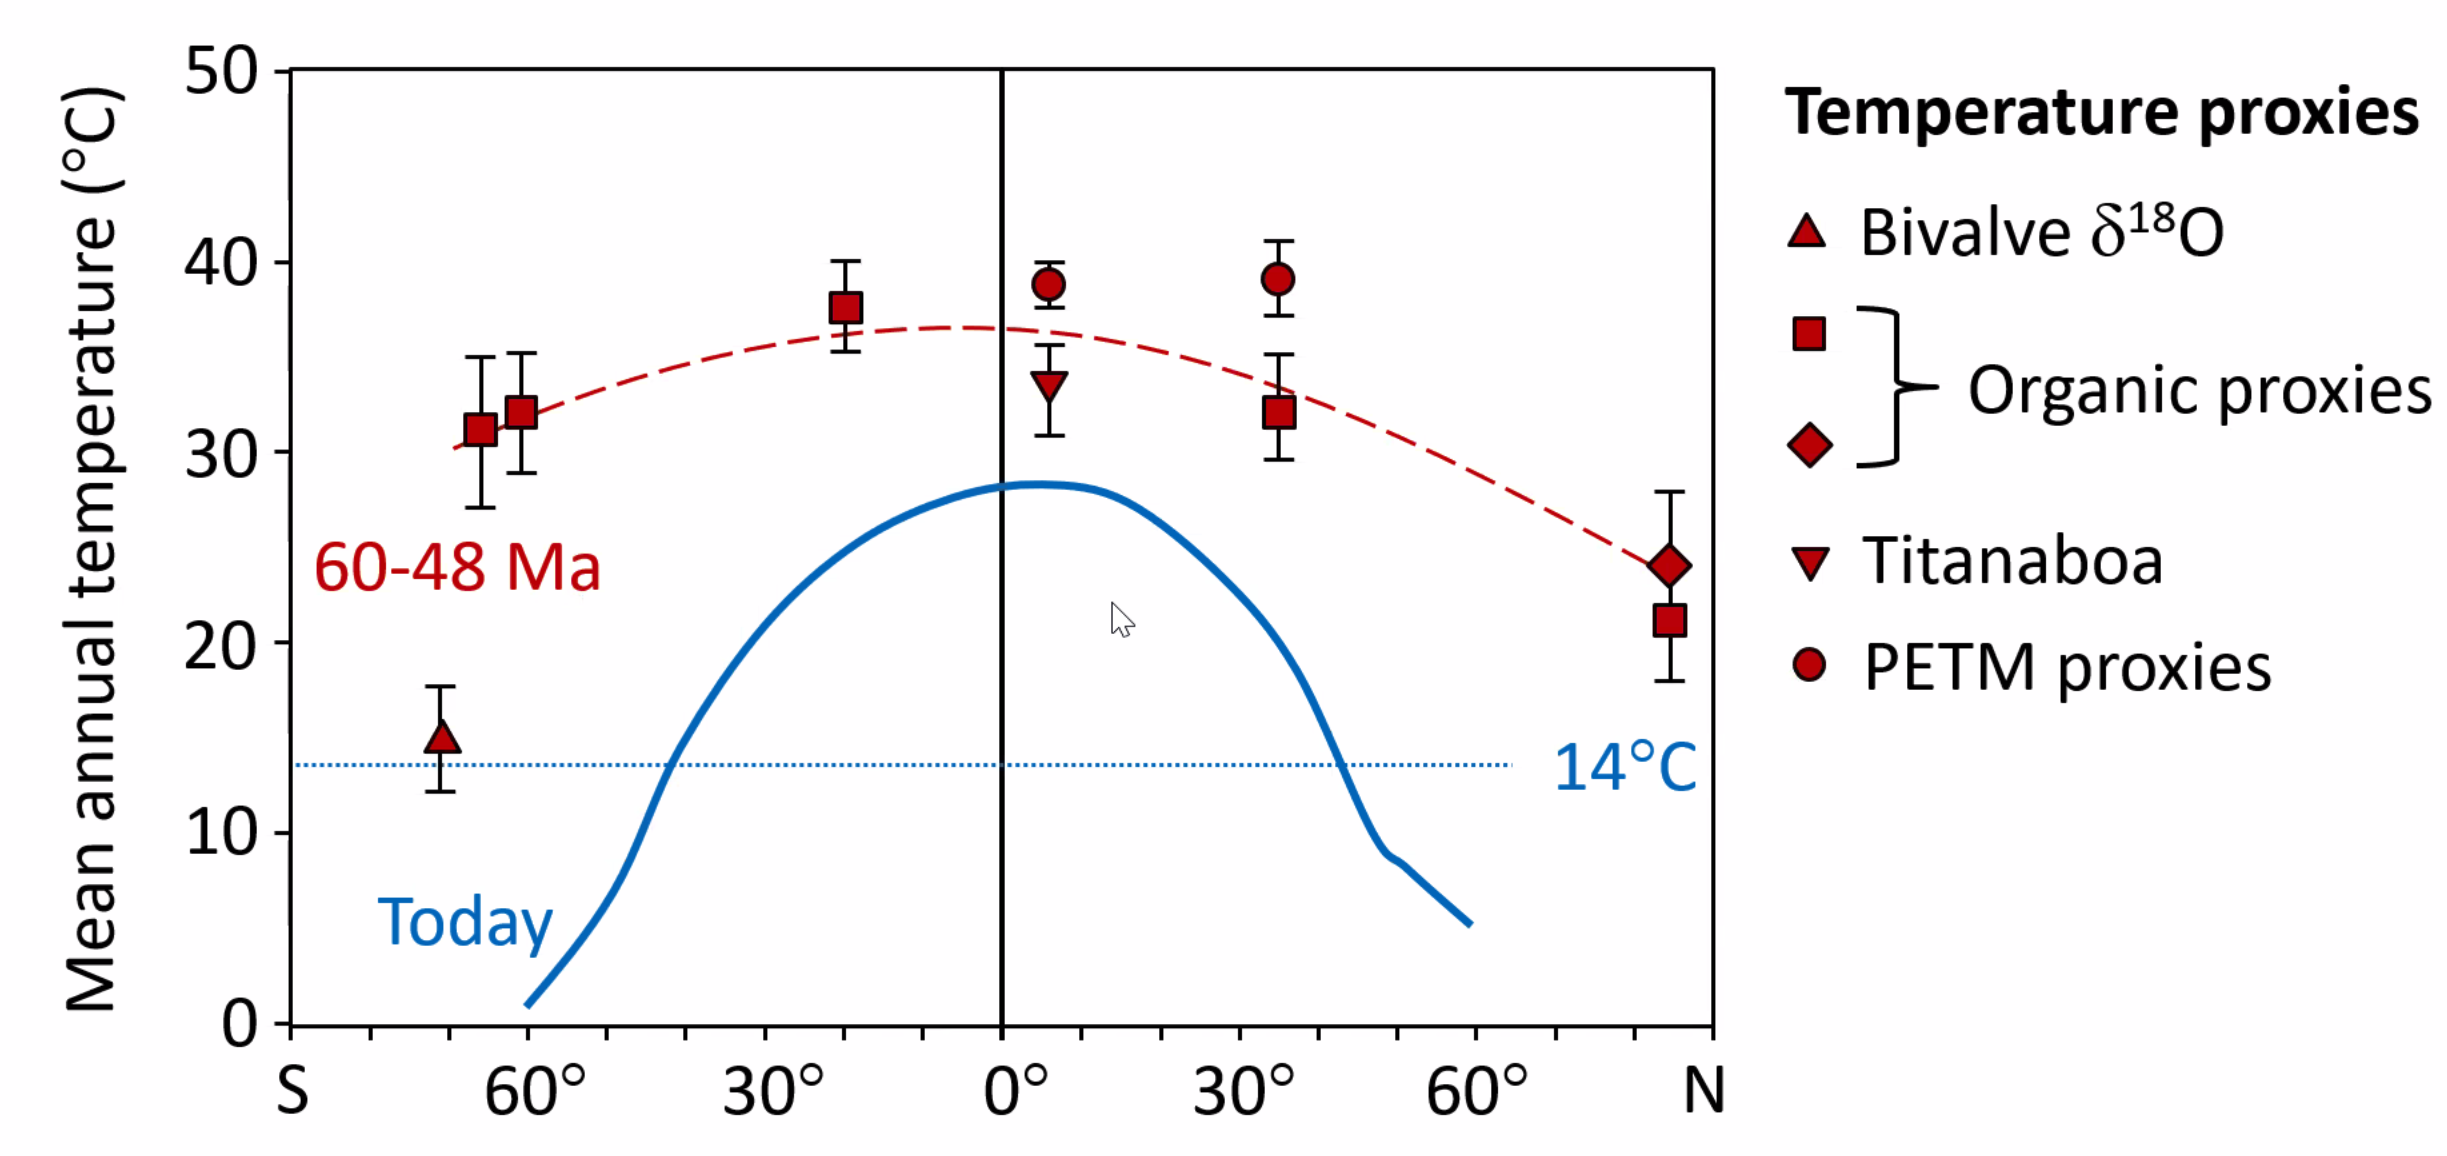
\includegraphics[width=0.75\linewidth]
    {content/img/temperature_proxies_warming.png}
\end{figure}

\subsection{Carbon isotope record: PETM}

Carbon isotope value becomes radically more negative at the PETM, mirroring the
oxygen data. Whatever was added to the ocean, must have a very negative
$\delta{13}C$.

Candidates:
\begin{itemize}
    \item Volcanoes ($CO_2$; $\delta{13}C = -6‰$)
    \item Methane from thawing of permafrost ($CH_4$; $\delta{13}C = -22‰$)
    \item Methane clathrates -- in sediments on
    a seafloor ($CH_4$; $\delta{13}C = -60‰$)
\end{itemize}

Was it a lot of volcanism, was it a fair amount of thawing permafrost, or was
it a little bit of methane clathrates?

$\delta^{13}C_{\text{source}} = [
(\delta^{13}C_2-\delta^{13}C_1) \times
(C_{\text{mass in ocean}} + C_{\text{mass added to ocean}})
-
(C_{\text{mass in ocean}} \times 1.5)
] / C_{\text{mass added to ocean}}$

We know the mass of carbon in the ocean to be 38700 billion tons.
We also know that $\delta^{13}C$ dropped from 1.5 to -1.5.

$\delta^{13}C_{\text{source}} = [
(-1.5-1.5) \times
(38700 + C_{\text{mass added to ocean}})
-
(38700 \times 1.5)
] / C_{\text{mass added to ocean}}$

Here's how much carbon we would need to add from different sources:

\begin{figure}[H]
    \centering
    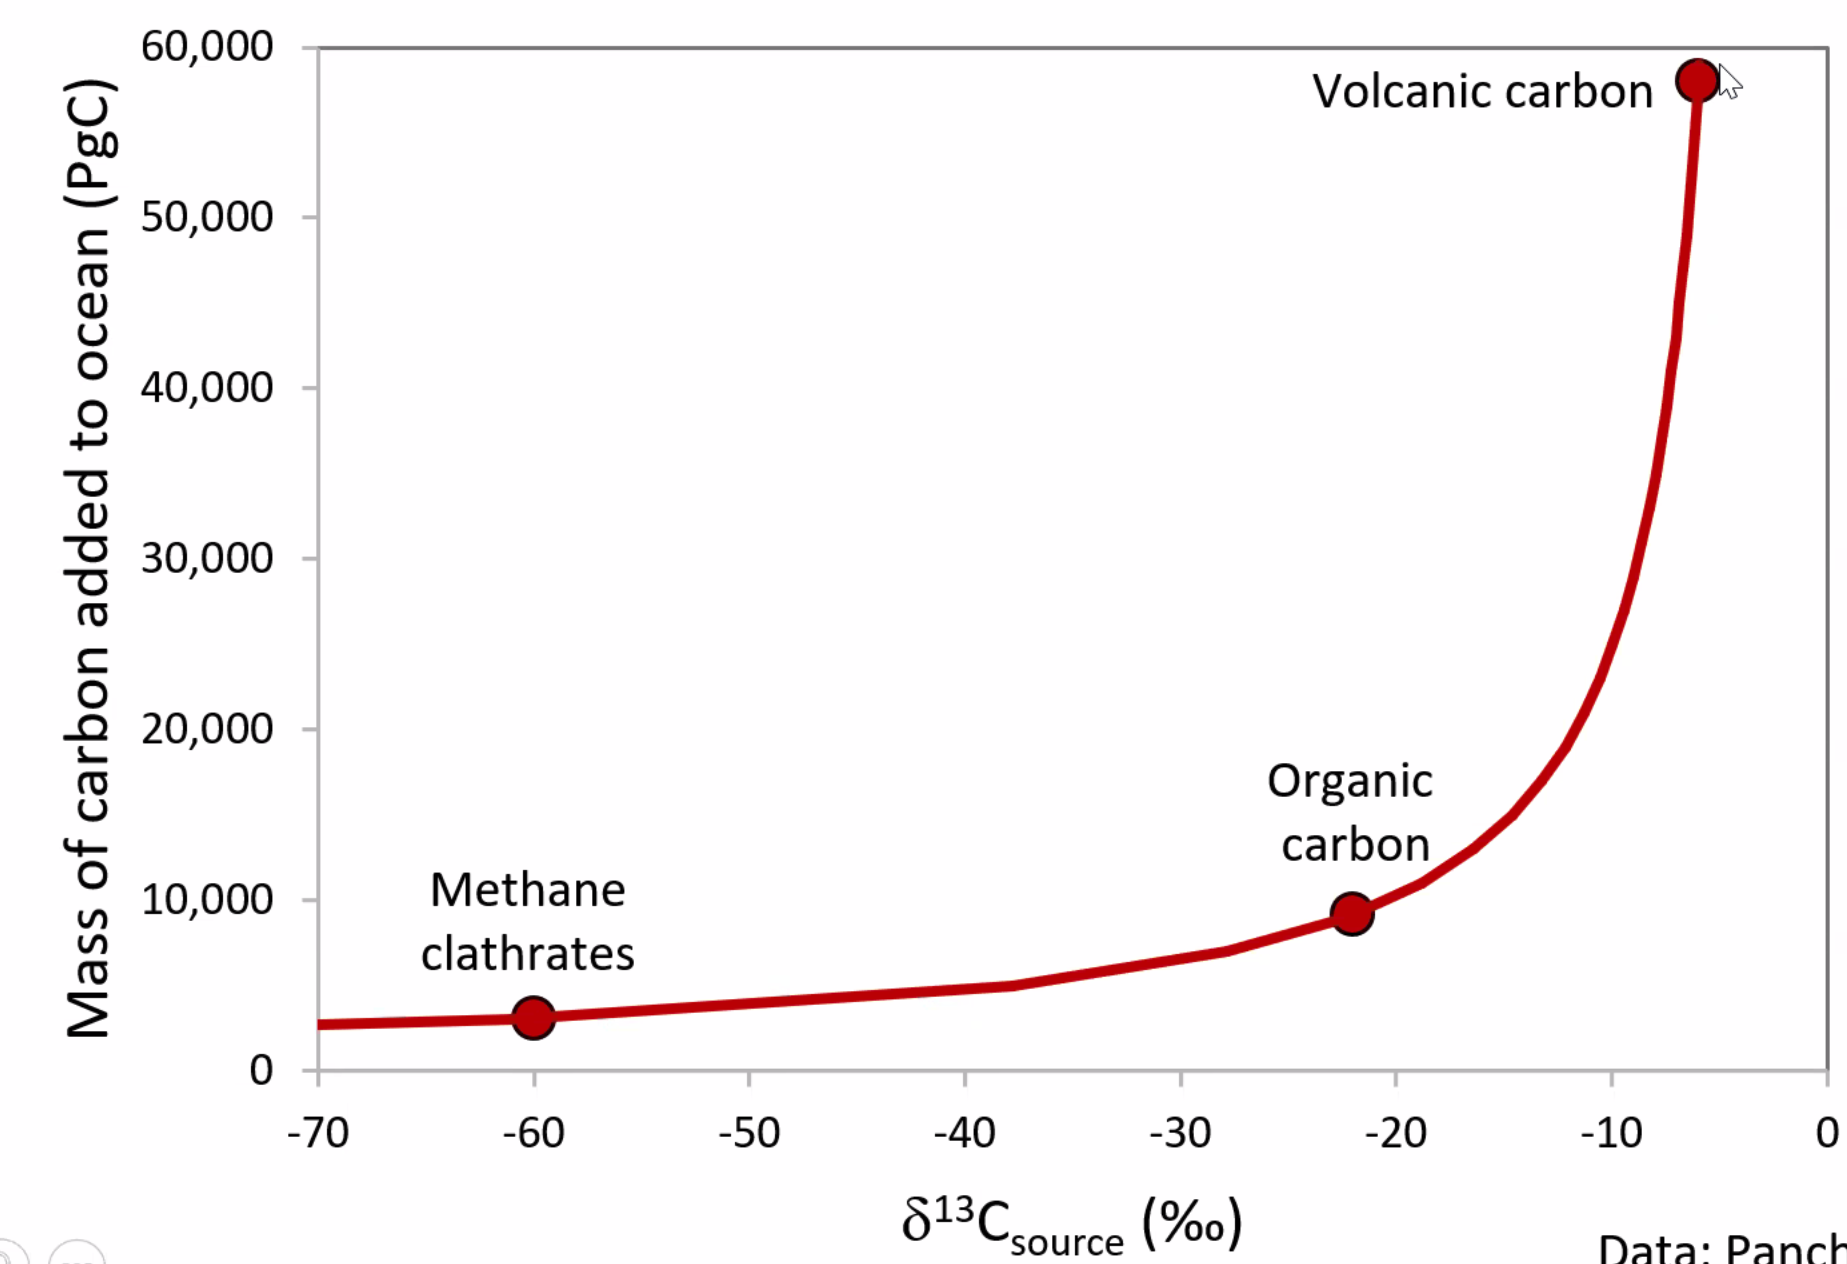
\includegraphics[width=0.75\linewidth]
    {content/img/adding_carbon_to_ocean.png}
\end{figure}

Researchers estimated that between 3000 PgC and 7126 PgC could have accumulated
in the ocean. This suggests that the likely source of carbon is not volcanoes,
simply not enough carbon is added. It must be one of the other two factors, or
the combination (thawing of permafrost or methane clathrates).

\subsection{Hypothesis}

More CO2 in the atmosphere and oceans because of volcanism
$\rightarrow$
Global warming
$\rightarrow$
Permafrost and/or methane clathrates thaw
$\rightarrow$
More CH$_4$/CO$_2$ in the atmosphere and oceans
$\rightarrow$
Greenhouse effect strengthens
$\rightarrow$
Global warming

The hypothesis is then that the \textbf{volcanism was the trigger} but the
thawing of permafrost and/or clathrates was the \textbf{feedback loop}.

\subsection{Carbonate Compensation Depth (CCD)}

CCD describes the depth at which the reaction swaps directions
$Ca^{2+} + 2 HCO_3^{-} \rightarrow CaCO_3 + CO2 + H_2O$\\
------------------------------ (CCD) --------------------------\\
$CaCO_3 + CO2 + H_2O \rightarrow Ca^{2+} + 2 HCO_3^{-}$

Beyond compensation depth, limestone dissolves.

When we add CO$_2$, the CCD rises to a higher level, because the bottom
reaction is favoured.

Currently, CCD is around 3500-4000 meters.

\subsection{Duration of PETM}

170000 years

That's how long it takes to recover after a perturbation of the carbon cycle.
That's important to know because people are perturbing the carbon cycle today.

\subsection{Bighorn Basin, Wyoming}
\begin{itemize}
    \item 5 species found only before PETM
    \item 22 species found before and after PETM
    \item 46 immigrant species during PETM
    \item 5 immigrant species after PETM
\end{itemize}

We're seeing this today, at $1.5 \degree$ warming, 2\% of species are heading
towards extinction.

%%%%%%%%%%%%%%%%%%%%%%%%%%%%%%%%%%%%%%%%%%%%%%%%%%%%%%%%%%%%%%%%%%%%%%%%%%%%%%%%